% !TeX root = construct.tex


\selectlanguage{hebrew}
\chapter{אמא'לה, המחוגה שלי התמוטטה!}\label{c.collapse}

%%%%%%%%%%%%%%%%%%%%%%%%%%%%%%%%%%%%%%%%%%%%%%%%%%%%%%%%%%%%%%%

\section{
\R{מחוגה קבועה ומחוגה מתמוטטת}
}

במחוגה מודרנית ניתן לקבע את המרחק בין הרגליים, וכך להעתיק קטע קו או מעגל ממקום למקום. נקרא למחוגה זו: "מחוגה קבועה". ראיתי בספרי לימוד גיאומטריה המציגים בניית אנך אמצעי של קטע קו על ידי בניית שני מעגלים עם רדיוסים שווים שמרכזם נקודות הקצה של הקו, ובלבד שהרדיוסים
\textbf{גדלים ממחצית אורך הקטע},
כפי שניתן לראות בתרשים השמאלי:
\begin{center}
\selectlanguage{english}
\begin{tikzpicture}[scale=0.5]
\begin{scope}
\coordinate (A) at (0,0);
\coordinate (B) at (4,0);
\draw (A) node[below left] {$A$} -- (B) node[below right] {$B$};
\fill (A) circle[radius=3pt];
\fill (B) circle[radius=3pt];
\draw[name path=larc] (A) ++(-60:3cm) arc (-60:60:3cm);
\draw[name path=rarc] (B) ++(-120:3cm) arc (-120:-240:3cm);
\path [name intersections={of=larc and rarc,by={b,t}}];
\fill (t) node[above right,xshift=-2pt,yshift=5pt] {$C$} circle[radius=3pt];
\fill (b) node[below left,xshift=2pt,yshift=-5pt] {$D$} circle[radius=3pt];
\draw ($ (b) ! 1.2 ! (t)$) -- ($ (t) ! 1.2 ! (b)$);
\end{scope}
\begin{scope}[xshift=12cm]
\coordinate (A) at (0,0);
\coordinate (B) at (4,0);
\draw (A) node[below left] {$A$} -- (B) node[below right] {$B$};
\fill (A) circle[radius=3pt];
\fill (B) circle[radius=3pt];
\draw[name path=larc] (A) ++(-80:4cm) arc (-80:80:4cm);
\draw[name path=rarc] (B) ++(-100:4cm) arc (-100:-260:4cm);
\path [name intersections={of=larc and rarc,by={b,t}}];
\fill (t) node[above right,xshift=-2pt,yshift=3pt] {$C$} circle[radius=3pt];
\fill (b) node[below left,xshift=2pt,yshift=-3pt] {$D$}circle[radius=3pt];
\draw ($ (b) ! 1.2 ! (t)$) -- ($ (t) ! 1.2 ! (b)$);
\end{scope}
\end{tikzpicture}
\end{center}

אוקלידס השתמש במחוגה "מתמוטטת" )%
\L{collapsing}%
(,
שרגליה מתקפלות כאשר מרימים אותה מהנייר. מחוגה המורכבת מגיר הקשור לחוט היא מחוגה מתמוטטת, כי אי-אפשר לשמור את הרדיוס כאשר מרימים אותה מהלוח. התרשים הימני למעלה מראה בנייה של אנך אמצעי באמצעות מחוגה מתמוטטת: האורך של
$AB$
שווה כמובן לאורך של
$BA$,
ולכן הרדיוסים של המעגלים שווים ללא צורך להעביר אורך קטע ממקום למקום.



ההוכחה שהקו שנבנה הוא האנך האמצעי לא פשוטה, כי צריך להשתמש במושגים יחסית מתקדמים כגון משולשים חופפים. באותה הבנייה נותנת משולש שווה צלעות )תרשים מימין(:

\vspace{-2ex}

\begin{center}
\selectlanguage{english}
\begin{tikzpicture}[scale=0.5]
\begin{scope}
\coordinate (A) at (0,0);
\coordinate (B) at (4,0);
\draw (A) node[below left] {$A$} -- (B) node[below right] {$B$};
\fill (A) circle[radius=3pt];
\fill (B) circle[radius=3pt];
\draw[name path=larc] (A) ++(-60:3cm) arc (-60:60:3cm);
\draw[name path=rarc] (B) ++(-120:3cm) arc (-120:-240:3cm);
\path [name intersections={of=larc and rarc,by={b,t}}];
\fill (t) node[above right,xshift=-2pt,yshift=5pt] {$C$} circle[radius=3pt];
\fill (b) node[below left,xshift=2pt,yshift=-5pt] {$D$} circle[radius=3pt];
\draw (A) -- (t);
\draw (B) -- (t);
\end{scope}
\begin{scope}[xshift=12cm]
\coordinate (A) at (0,0);
\coordinate (B) at (4,0);
\draw (A) node[below left] {$A$} -- (B) node[below right] {$B$};
\fill (A) circle[radius=3pt];
\fill (B) circle[radius=3pt];
\draw[name path=larc] (A) ++(-80:4cm) arc (-80:80:4cm);
\draw[name path=rarc] (B) ++(-100:4cm) arc (-100:-260:4cm);
\path [name intersections={of=larc and rarc,by={b,t}}];
\fill (t) node[above right,xshift=-2pt,yshift=3pt] {$C$} circle[radius=3pt];
\fill (b) node[below left,xshift=2pt,yshift=-3pt] {$D$}circle[radius=3pt];
\draw (A) -- (t);
\draw (B) -- (t);
\end{scope}
\end{tikzpicture}
\end{center}

\vspace{-2ex}
ההוכחה פשוטה: אורך הקטע
$AC$
שווה לאורך הקטע
$AB$
כי שניהם רדיוסים של אותו מעגל, ומאותה סיבה האורך של
$BC$
שווה לאורך של
$BA$.
מכאן:
\[
AC = AB = BA = BC\,.
\]
התרשים משמאל מראה שהבנייה עם מחוגה קבועה ורדיוסים שרירותיים נותנת משולש שווה שוקיים שהוא לא בהכרח משולש שווה צלעות.

\np

בנייה זו של משולש שווה צלעות היא המשפט הראשון בספר "יסודות" של אוקלידס. המשפט השני בספר מראה שאפשר להעתיק קטע קו נתון
$AB$
לקטע קו שאחת מנקודות הקצה שלה היא נקודה נתונה
$C$.
אם בונים מעגל שמרכזו
$C$
והרדיוס שלו הוא העותק של
$AB$,
מתקבל עותק של מעגל נתון שמרכזו 
$A$
והרדיוס שלו
$AB$.
המסקנה היא שלכל בנייה באמצעות מחוגה קבועה, קיימת בנייה שקולה באמצעות מחוגה מתמוטטת.

במאמר מרתק 
\L{\cite{toussaint}}, 
\L{Godfried Toussaint}
מראה שפורסמו הוכחות שגויות רבות של המשפט, ודווקא אוקלידס הוא זה שנתן הוכחה נכונה! במסמך זה, אביא את הבנייה של אוקלידס בשלבים, ביחד עם הוכחת הנכונות, ואחר כך בנייה שגויה שניתן למצוא אפילו בספרים שפרוסמו לאחרונה. אחר כך, אסקור כלים מורכבים יותר לבנייה גיאומטרית. לבסוף, אביא הוכחה
\textbf{שכל}
משולש הוא שווה שוקיים כדי לראות שאי-אפשר לסמוך על תרשים.

%%%%%%%%%%%%%%%%%%%%%%%%%%%%%%%%%%%%%%%%%%%%%%%%%%%%%%%%%%%%%%%

\section{%
העתקת קטע קו לפי אוקלידס%
}

\textbf{משפט}
\L{(Compasss Equivalency Theorem)}:
נתון קטע קו
$AB$
ונקודה
$C$
)תרשים משמאל(, ניתן לבנות )עם מחוגה מתמוטטת( בנקודה
$C$
קטע קו שאורכו שווה לאורכו של 
$AB$:


\begin{center}
\selectlanguage{english}
\begin{tikzpicture}[scale=0.4]
\begin{scope}
\coordinate (C) at (0,0);
\coordinate (A) at (2.5,0);
\coordinate (B) at (5.5,2);
\draw (A) node[below,xshift=-2pt,yshift=-2pt] {$A$} -- (B) node[right] {$B$};
\fill (A) circle[radius=3pt];
\fill (B) circle[radius=3pt];
\fill (C) node[below,xshift=2pt,yshift=-2pt] {$C$} circle[radius=3pt];
\end{scope}
\begin{scope}[xshift=12cm]
\coordinate (C) at (0,0);
\coordinate (A) at (2.5,0);
\coordinate (B) at (5.5,2);
\draw (A) node[below,xshift=-2pt,yshift=-2pt] {$A$} -- (B) node[right] {$B$};
\fill (A) circle[radius=3pt];
\fill (B) circle[radius=3pt];
\fill (C) node[below,xshift=2pt,yshift=-2pt] {$C$} circle[radius=3pt];
\draw (A) -- (C);
\path[name path=larc] (C) ++(-70:2.5cm) arc (-70:70:2.5cm);
\path[name path=rarc] (A) ++(-110:2.5cm) arc (-110:-250:2.5cm);
\path [name intersections={of=larc and rarc,by={d,D}}];
\fill (D) node[above] {$D$} circle[radius=3pt];
\draw (A) -- (D);
\draw (C) -- (D);
\end{scope}
\end{tikzpicture}
\end{center}

\vspace*{-6ex}
\textbf{%
הבנייה:%
}

חבר בקו את הנקודות
$A$
ו-%
$C$.

בנה משולש שווה צלעות שבסיסו
$AC$. 
המשפט הראשון של אוקלידס מראה את הבנייה עם מחוגה מתמוטטת. סמן את הקודקוד של המשולש ב-%
$D$
)תרשים ימני למעלה(. 

בנה קרן בהמשך של
$DA$
וקרן בהמשך של 
$DC$
)התרשים משמאל(:

\begin{center}
\selectlanguage{english}
\begin{tikzpicture}[scale=0.4]
\begin{scope}
\coordinate (C) at (0,0);
\coordinate (A) at (2.5,0);
\coordinate (B) at (5.5,2);
\draw (A) node[below,xshift=-2pt,yshift=-2pt] {$A$} -- (B) node[right] {$B$};
\fill (A) circle[radius=3pt];
\fill (B) circle[radius=3pt];
\fill (C) node[below,xshift=2pt,yshift=-2pt] {$C$} circle[radius=3pt];
\draw (A) -- (C);
\path[name path=larc] (C) ++(-70:2.5cm) arc (-70:70:2.5cm);
\path[name path=rarc] (A) ++(-110:2.5cm) arc (-110:-250:2.5cm);
\path [name intersections={of=larc and rarc,by={d,D}}];
\fill (D) node[above] {$D$} circle[radius=3pt];
\draw (A) -- (D);
\draw (C) -- (D);
\draw[name path=ray2] (D) -- ($ (D) ! 3 ! (C) $);
\draw[name path=ray1] (D) -- ($ (D) ! 3 ! (A) $);
\end{scope}
\begin{scope}[xshift=12cm]
\coordinate (C) at (0,0);
\coordinate (A) at (2.5,0);
\coordinate (B) at (5.5,2);
\draw (A) node[below,xshift=-2pt,yshift=-2pt] {$A$} -- (B) node[right] {$B$};
\fill (A) circle[radius=3pt];
\fill (B) circle[radius=3pt];
\fill (C) node[below,xshift=2pt,yshift=-2pt] {$C$} circle[radius=3pt];
\draw (A) -- (C);
\path[name path=larc] (C) ++(-70:2.5cm) arc (-70:70:2.5cm);
\path[name path=rarc] (A) ++(-110:2.5cm) arc (-110:-250:2.5cm);
\path [name intersections={of=larc and rarc,by={d,D}}];
\fill (D) node[above] {$D$} circle[radius=3pt];
\draw (A) -- (D);
\draw (C) -- (D);
\draw[name path=ray2] (D) -- ($ (D) ! 3 ! (C) $);
\draw[name path=ray1] (D) -- ($ (D) ! 3 ! (A) $);
\node[draw,circle through=(B),name path=c1] at (A) {};
\path [name intersections={of=c1 and ray1,by={E,e}}];
\fill (E) node[right,xshift=2pt,yshift=-2pt] {$E$} circle[radius=3pt];
\end{scope}
\end{tikzpicture}
\end{center}


בנה מעגל שמרכזו 
$A$
עם רדיוס
$AB$.
$E$
הוא החיתוך של המעגל עם הקרן
$DE$
)תרשים מימין(.

בנה מעגל שמרכזו 
$D$
עם רדיוס 
$DC$.
סמן את החיתוך של הקרן
$DC$
עם המעגל ב-%
$F$:

\np

\begin{center}
\selectlanguage{english}
\begin{tikzpicture}[scale=0.4]
\coordinate (C) at (0,0);
\coordinate (A) at (2.5,0);
\coordinate (B) at (5.5,2);
\draw (A) node[below,xshift=-2pt,yshift=-2pt] {$A$} -- node[above] {$x$} (B) node[right] {$B$};
\fill (A) circle[radius=3pt];
\fill (B) circle[radius=3pt];
\fill (C) node[below,xshift=2pt,yshift=-2pt] {$C$} circle[radius=3pt];
\draw (A) -- (C);
\path[name path=larc] (C) ++(-70:2.5cm) arc (-70:70:2.5cm);
\path[name path=rarc] (A) ++(-110:2.5cm) arc (-110:-250:2.5cm);
\path [name intersections={of=larc and rarc,by={d,D}}];
\fill (D) node[above] {$D$} circle[radius=3pt];
\draw (A) -- node[right] {$y$} (D);
\draw (C) -- node[left] {$y$} (D);
\draw[name path=ray2] (D) -- ($ (D) ! 3 ! (C) $);
\draw[name path=ray1] (D) -- ($ (D) ! 3 ! (A) $);
\node[draw,circle through=(B),name path=c1] at (A) {};
\path [name intersections={of=c1 and ray1,by={E,e}}];
\fill (E) node[right,xshift=2pt,yshift=-2pt] {$E$} circle[radius=3pt];
\node[draw,circle through=(E),name path=c2] at (D) {};
\path [name intersections={of=c2 and ray2,by={F,f}}];
\fill (F) node[left,xshift=-2pt,yshift=-2pt] {$F$} circle[radius=3pt];
\path (A) -- node[right] {$x$} (E);
\path (C) -- node[left] {$x$} (F);
\end{tikzpicture}
\end{center}

\textbf{טענה:}
אורכו של קטע הקו
$CF$
שווה לאורך קטע הקו
$AB$.

%\vspace*{-7ex}
\textbf{הוכחה:}
$DC=DA$
כי
$\triangle ACD$
שווה צלעות.
$AE=AB$
כי שניהם רדיוסים של המעגל שמרכזו 
$A$.
$DF=DE$
כי שניהם רדיוסים של המעגל שמרכזו
$D$.
לכן, אורך קטע הקו 
$CF$ 
הוא:
\[
CF = DF - DC = DE - DC = DE - DA = AE = AB\,.
\].

%%%%%%%%%%%%%%%%%%%%%%%%%%%%%%%%%%%%%%%%%%%%%%%%%%%%%%%%%%%%%%%

\vspace{-8ex}

\section{%
העתקה שגויה של קטע קו
}\label{sec.error}

\hspace{-8pt}
\textbf{
משפט
\L{(Compasss Equivalency Theorem)}:
}
נתון קטע קו
$AB$
ונקודה
$C$,
ניתן לבנות )באמצעות מחוגה מתמוטטת( בנקודה
$C$
קטע קו שאורכו שווה לאורכו של 
$AB$.

\textbf{בנייה}
\L{(\cite{rusty})}:
%\vspace*{-2ex}

בנה מעגל שמרכזו 
$A$
עם רדיוס
$AB$:

\begin{center}
\selectlanguage{english}
\begin{tikzpicture}[scale=0.4]
\begin{scope}
\coordinate (C) at (-2,0);
\coordinate (A) at (2.5,0);
\coordinate (B) at (4.5,1.5);
\draw (A) node[below,xshift=-2pt,yshift=-2pt] {$A$} -- (B) node[right] {$B$};
\fill (A) circle[radius=3pt];
\fill (B) circle[radius=3pt];
\fill (C) node[below,xshift=2pt,yshift=-2pt] {$C$} circle[radius=3pt];
\end{scope}
\begin{scope}[xshift=12cm]
\coordinate (C) at (-2,0);
\coordinate (A) at (2.5,0);
\coordinate (B) at (4.5,1.5);
\draw (A) node[below,xshift=-2pt,yshift=-2pt] {$A$} -- (B) node[right] {$B$};
\fill (A) circle[radius=3pt];
\fill (B) circle[radius=3pt];
\fill (C) node[below,xshift=2pt,yshift=-2pt] {$C$} circle[radius=3pt];
\node[draw,circle through=(B),name path=c1] at (A) {};
\end{scope}
\end{tikzpicture}
\end{center}
%\vspace*{-8ex}

בנה מעגל שמרכזו
$A$
עם רדיוס
$AC$
ומעגל שמרכזו
$C$
עם רדיוס
$AC=CA$.
סמן את נקודות החיתוך של המעגלים ב-%
$E,F$,
וסמן את החיתוך של המעגל שמרכזו
$C$
עם המעגל שמרכזו
$A$
ב-%
$D$.

\begin{center}
\selectlanguage{english}
\begin{tikzpicture}[scale=0.4]
\coordinate (C) at (-2,0);
\coordinate (A) at (2.5,0);
\coordinate (B) at (4.5,1.5);
\draw (A) node[below right] {$A$} -- (B) node[right] {$B$};
\fill (A) circle[radius=3pt];
\fill (B) circle[radius=3pt];
\fill (C) node[left,xshift=-2pt] {$C$} circle[radius=3pt];
\node[draw,circle through=(B),name path=c1] at (A) {};
\node[draw,circle through=(C),name path=c2] at (A) {};
\node[draw,circle through=(A),name path=c3] at (C) {};
\path [name intersections={of=c1 and c3,by={D,f}}];
\path [name intersections={of=c2 and c3,by={E,F}}];
\fill (D) node[below right,xshift=4pt] {$D$} circle[radius=3pt];
\fill (E) node[above,yshift=2pt] {$E$} circle[radius=3pt];
\fill (F) node[below,yshift=-2pt] {$F$} circle[radius=3pt];
\end{tikzpicture}
\end{center}

בנה מעגל שמרכזו 
$E$
עם רדיוס 
$ED$.
סמן את החיתוך של מעגל זה עם המעגל שמרכזו
$C$
ב-%
$G$.
ארכו של קטע הקו 
$GC$
שווה לאורכו של
$AB$.

\np

\begin{center}
\selectlanguage{english}
\begin{tikzpicture}[scale=0.4]
\coordinate (C) at (-2,0);
\coordinate (A) at (2.5,0);
\coordinate (B) at (4.5,1.5);
\draw (A) node[below right] {$A$} -- (B) node[right] {$B$};
\fill (A) circle[radius=3pt];
\fill (B) circle[radius=3pt];
\fill (C) node[below left] {$C$} circle[radius=3pt];
\node[draw,circle through=(B),name path=c1] at (A) {};
\node[draw,circle through=(C),name path=c2] at (A) {};
\node[draw,circle through=(A),name path=c3] at (C) {};
\path [name intersections={of=c1 and c3,by={D,f}}];
\path [name intersections={of=c2 and c3,by={E,F}}];
\fill (D) node[below right,xshift=4pt] {$D$} circle[radius=3pt];
\fill (E) node[above,yshift=2pt] {$E$} circle[radius=3pt];
\fill (F) node[below,yshift=-2pt] {$F$} circle[radius=3pt];
\node[draw,circle through=(D),name path=c4] at (E) {};
\path [name intersections={of=c2 and c4,by={g,G}}];
\fill (G) node[below left,xshift=-4pt] {$G$} circle[radius=3pt];
\draw (C) -- (G);
\draw[dashed] (G) -- (E) -- (C);
\draw[dashed] (A) -- (D) -- (E) -- cycle;
\end{tikzpicture}
\end{center}

חשוב להשתכנע שהבנייה אפשרית עם מחוגה מתמוטטת.

את ההוכחה ש-%
$AB=GC$
ניתן למצוא ב-%
\L{\cite{rusty}}.
בהוכחה יש להראות ששני המשולשים המסומנים בקווים במקוקווים חופפים כך ש-%
$GC=DA=AB$.
ההוכחה ארוכה הרבה יותר מההוכחה של אוקלידס ומשתמשת במושגים מתקדמים יחסית להוכחה של אוקלידס המשתמשת רק במושגים: כל הרדיוסים של מעגל שווים וכל הצלעות של משולש שווה צלעות שווים.

עברו בעיון על ההוכחה ב-%
\cite{rusty}
ש-%
$AB=GC$
וחפש את השגיאה. התשובה: אין שום שגיאה בהוכחה! השגיאה נובעת ממקור אחר: השווין
$AB=GC$
מתקיים רק כאשר אורכו של 
$AB$
קטן מאורכו של
$AC$.
הבנייה של אוקלידס נכונה ללא קשר לאורך היחסי של הקווים ולמיקום של הנקודה
$C$
ביחס לקטע הקו
$AB$
)\cite{toussaint}(.

%%%%%%%%%%%%%%%%%%%%%%%%%%%%%%%%%%%%%%%%%%%%%%%%%%%%%%%%%%%%%%%
\begin{comment}
\section{%
חקר הבניות עם גיאוגברה%
}
הכנתי קבצי גיאוגברה עבור שתי הבניות:
\begin{center}
\L{\texttt{compass-equivalency.ggb, rusty-compass.ggb}}.
\end{center}
ניתן להזיז את הנקודות
$A,B,C$
כדי לראות איך הציור משתנה, ולמדוד את שני אורכים כדי לבדוק אם הם שווים.

\textbf{%
שימו לב:%
}
בבנייה של אוקלידס, אם מתחילים עם 
$AB<AC$,
מזיזים את
$C$
כך ש-%
$AB>AC$
וחוזרים, התצוגה מתקלקלת. הסיבה היא שכאשר
$AB<AB$,
לקרן
$DA$
יש שתי נקודות חיתוך עם המעגל שמרכזו
$A$.
כאשר חוזרים למצב ש-%
$AB<AC$
נאבד נקודת החיתוך. כדי להתגבר על הבעייה הכנתי שני קבצים עבור שני מצבים.

\end{comment}
%%%%%%%%%%%%%%%%%%%%%%%%%%%%%%%%%%%%%%%%%%%%%%%%%%%%%%%%%%%%%%%

\section{
דרך "פשוטה יותר" להעתקת מעגל
}

נתון קטע קו 
$AB$
ונקודה
$C$,
אם נוכל לבנות מקבילית כאשר שלושת הנקודות הן קודקודים, נקבל קטע קו עם 
$C$
בקצה אחד שאורכו שווה לאורכו של
$AB$
)תרשים שמאלי(. ראו
\L{\cite[%
207--208
\R{עמ'}%
]{roads}}.

\begin{center}
\selectlanguage{english}
\begin{tikzpicture}[scale=0.6]
\coordinate (A) at (0,0);
\coordinate (B) at (4,0);
\coordinate (C) at (5,2);
\draw (A) -- (B);
\path (A) -- node[above] {$x$} (B);
\fill (A) node[below] {$A$} circle[radius=3pt];
\fill (B) node[below] {$B$} circle[radius=3pt];
\fill (C) node[above] {$C$} circle[radius=3pt];
\draw (B) -- node[right] {$y$} (C);
\coordinate (D) at ($(C)+(-40mm,0cm)$);
\draw (D) -- node[above] {$x$} (C);
\draw (A) -- node[left] {$y$} (D);
\fill (D) node[above] {$D$} circle[radius=3pt];
\begin{scope}[xshift=12cm]
\coordinate (A) at (0,0);
\coordinate (B) at (4,0);
\coordinate (C) at (5,2);
\draw ($ (B) ! 1.2 ! (A) $) -- ($ (A) ! 1.5 ! (B) $);
\path (A) -- (B);
\fill (A) node[below right] {$A$} circle[radius=3pt];
\fill (B) node[below] {$B$} circle[radius=3pt];
\fill (C) node[above] {$C$} circle[radius=3pt];
\draw (B) -- (C);
\draw[name path=ray1] ($(C)+(-5cm,0cm)$) -- ($(C)+(1cm,0cm)$);
\draw[name path=ray2] ($(A)+(-.25,-.65)$) -- ($(A)+(1,2.6)$);
\path [name intersections={of=ray1 and ray2,by={E}}];
\fill (E) node[above left] {$E$} circle[radius=3pt];
\coordinate (D) at (C |- B);
\draw (C) -- (D);
\fill (D) node[below] {$D$} circle[radius=3pt];
\end{scope}
\end{tikzpicture}
\end{center}

\textbf{בנייה} 
)תרשים מימין(:


חבר את
$B$
ו-%
$C$.

בנה אנך מ-%
$C$
לקו המכיל את הקטע
$AB$.
נסמן את נקודת החיתוך ב-%
$D$.

בנה אנך לקטע
$CD$
מהנקודה
$C$.
הקו המכיל את האנך מקביל ל-%
$AB$.

באותה דרך בנה קו המקביל ל-%
$BC$
דרך 
$A$. 
נסמן את נקודת החיתוך של שני הקווים ב-%
$E$.

אורכו של קטע הקו
$EC$
שווה לאורכו של
$AB$
ו-%
$C$
היא נקודת קצה שלו.


יש לוודא שאפשר לבנות את המקבילית עם מחוגה מתמוטטת. למעשה, הבנייה יחידה הנחוצה היא של אנך מנקודה שרירותית נתונה לקו המכיל קטע קו נתון:

\np

\begin{center}
\selectlanguage{english}
\begin{tikzpicture}[scale=0.5]
\coordinate (A) at (0,0);
\coordinate (B) at (4,0);
\coordinate (C) at (5,2);
\draw ($ (B) ! 1.5 ! (A) $) -- ($ (A) ! 1.5 ! (B) $);
\fill (A) node[below] {$A$} circle[radius=3pt];
\fill (B) node[below] {$B$} circle[radius=3pt];
\fill (C) node[right] {$C$} circle[radius=3pt];
\end{tikzpicture}
\end{center}

נבנה מעגל שמרכזו
$C$
עם רדיוס הגדול מהמרחק של
$C$
מהקו:
\begin{center}
\selectlanguage{english}
\begin{tikzpicture}[scale=0.5]
\coordinate (A) at (0,0);
\coordinate (B) at (4,0);
\coordinate (C) at (5,2);
\draw[name path=ray] ($ (B) ! 1.5 ! (A) $) -- ($ (A) ! 2.5 ! (B) $);
\fill (A) node[below] {$A$} circle[radius=3pt];
\fill (B) node[below] {$B$} circle[radius=3pt];
\fill (C) node[right] {$C$} circle[radius=3pt];
\draw[name path=arc] (C) ++(-160:3.5cm) arc (-160:-20:3.5cm);
\path [name intersections={of=arc and ray,by={D,E}}];
\fill (D) node[below left] {$D$} circle[radius=3pt];
\fill (E) node[below right] {$E$} circle[radius=3pt];
\end{tikzpicture}
\end{center}


בנה אנך אמצעי ל-%
$DE$
דרך 
$C$.
$CD=CE$
כי הם שני רדיוסים שווים של אותו מעגל וניתן לבנות את האנך באמצעות מחוגה מתמוטטת:

\begin{center}
\selectlanguage{english}
\begin{tikzpicture}[scale=0.5]
\coordinate (A) at (0,0);
\coordinate (B) at (4,0);
\coordinate (C) at (5,2);
\draw[name path=ray] ($ (B) ! 1.5 ! (A) $) -- ($ (A) ! 2.5 ! (B) $);
\fill (A) node[below] {$A$} circle[radius=3pt];
\fill (B) node[below] {$B$} circle[radius=3pt];
\fill (C) node[right] {$C$} circle[radius=3pt];
\path[name path=arc] (C) ++(-160:3.5cm) arc (-160:-20:3.5cm);
\path [name intersections={of=arc and ray,by={D,E}}];
\fill (D) node[below left] {$D$} circle[radius=3pt];
\fill (E) node[below right] {$E$} circle[radius=3pt];
\draw[name path=larc] (D) ++(-60:3.5cm) arc (-60:60:3.5cm);
\draw[name path=rarc] (E) ++(-120:3.5cm) arc (-120:-240:3.5cm);
\path [name intersections={of=larc and rarc,by={b,t}}];
\fill (b) circle[radius=3pt];
\draw ($ (b) ! 1.2 ! (t)$) -- ($ (t) ! 1.2 ! (b)$);
\end{tikzpicture}
\end{center}

למה אוקלידס לא הביא בנייה זו? כפי שהזכרנו לעיל, הוכחת הנכונות של הבנייה של אנך אמצעי כלל לא פשוטה, בעוד הוכחת הנכונות של הבנייה של אוקלידס מסתמכת על משפט פשוט אחד.


%%%%%%%%%%%%%%%%%%%%%%%%%%%%%%%%%%%%%%%%%%%%%%%%%%%%%%%%%%%%%%%

\begin{comment}

\section{
הגבלות והרחבות של בנייה באמצעות סרגל ומחוגה
}

ראינו שמה שניתן לבנות עם סרגל ומחוגה קבועה ניתן לבנות עם סרגל ומחוגה מתקפלת. מתמטיקאים חקרו אפשרות מוגבלות יותר:

\begin{itemize}
\item
כל בנייה עם סרגל ומחוגה ניתנת לבנייה עם מחוגה בלבד! כמובן, אם אין סרגל לא נראה קווים, אבל שתי נקודות במישור מגדירות קו ואין צורך ממש לראות אותו. למשל, אם ניתנות שתי נקודות
$A,B$
אפשר לבנות עם מחוגה בלבד נקודה
$C$
שהמרחק שלה מ-%
$A$
ומ-%
$B$
שווה למרחק
$AB$
)איור~%
\ref{fig.mm}(.
בנינו משולש שווה צלעות, אמנם ללא צלעות. המשפט הוכח בשנת
\L{1672}
על ידי
\L{Georg Mohr}
ובאופן עצמאי בשנת
\L{1797}
על ידי
\L{Lorenzo Mascheroni}.
\begin{figure}[H]
\begin{center}
\selectlanguage{english}
\begin{tikzpicture}[scale=0.5]
\coordinate (A) at (0,0);
\coordinate (B) at (4,0);
\path (A) node[below left] {$A$} -- (B) node[below right] {$B$};
\fill (A) circle[radius=3pt];
\fill (B) circle[radius=3pt];
\draw[name path=larc] (A) ++(-10:4cm) arc (-10:80:4cm);
\draw[name path=rarc] (B) ++(-170:4cm) arc (-170:-260:4cm);
\path [name intersections={of=larc and rarc,by={t}}];
\fill (t) node[above] {$C$} circle[radius=3pt];
\end{tikzpicture}
\selectlanguage{hebrew}
\caption{%
בניית משלוש שווה צלעות עם מחוגה בלבד.%
}\label{fig.mm}
\end{center}
\end{figure}
\vspace*{-8ex}
\item
אי-אפשר להסתפק בסרגל בלבד, אבל אם קיים במישור מעגל אחד בלבד )לא משנה איפה מרכז המעגל או הרדיוס שלו(, ניתן לבנות את כל מה שאפשר לבנות עם סרגל ומחוגה. המשפט הוכח ב-%
\L{1833}
על ידי 
\L{Jacob Steiner}.
\end{itemize}
ההוכחות של שני המשפטים מעט ארוכות אבל לא מסובכות במיוחד. אפשר למצוא אותן בספרו של
\L{Heinrich D\"{o}rrie}
\L{\cite{dorrie1}}.
ספר זה נגיש יותר במהדורה חדשה 
\L{\cite{dorrie2}}.

בכיוון השני, היוונים חקרו מה אפשר לבנות אם משתמשים בכלים מורכבים יותר מסרגל )ללא סימנים( ומחוגה. במאה ה-%
\L{19}
הוכח שלא ניתן לחלק זווית לשלושה חלקים שווים באמצעות סרגל ומחוגה. ניתן לבצע את הבנייה עם סרגל בעל שני סימנים הנקרא
\L{neusis}
או עם מכשיר הנקרא
\L{quadratrix},
המורכב משני סרגלים המחוברים כך שהם יכולים לגלוש אחד ליד השני ולהסתובב. כתבתי מסמך המתאר את הבניות
\textbf{איך לחלק זווית לשלושה )אם אתם מוכנים לרמות(}
שניתן למצוא באתר שלי:\\
\selectlanguage{english}
\url{http://www.weizmann.ac.il/sciÎtea/benari/mathematics}.

\end{comment}
%%%%%%%%%%%%%%%%%%%%%%%%%%%%%%%%%%%%%%%%%%%%%%%%%%%%%%%%%%%%%%%

\selectlanguage{hebrew}

\section{
אין לסמוך על ציור
}
בסעיף~%
\ref{sec.error}
ראינו שאין לסמוך על ציור. הנה הוכחה "נכונה"
\textbf{\R{שכל}}
משולש שווה שוקיים!

נתון משולש שרירותי 
$ABC$,
תהי
$P$
נקודת החיתוך בין חוצה הזווית של
$\angle BAC$
לבין האנך האמצעי של 
$BC$.
סימנו ב-%
$D,E,F$
את נקודות החיתוך של האנחים מ-%
$P$
לצלעות
$BC,AB,AC$. $\triangle APE\cong \triangle APF$
כי הם משולשים ישר זווית עם זוויות שוות
$\alpha$
וצלע $AP$ משותף.

$\triangle DPB\cong \triangle DPC$
לפי צ.ז.צ. כי 
$PD$
הוא צלע משותף, ו-%
$BD=DC=a$
כי 
$PD$
הוא האנך האמצעי ל-%
$BC$.
$\triangle EPB\cong \triangle FPC$,
כי
$EP=PF$
לפי החפיפה הראשונה, ו-%
$PB=PC$
לפי החפיפה השנייה. נחבר את השוויונות ונקבל ש-%
$\triangle ABC$
שווה שוקיים:
\[
AB=AE+EB=AF+FC=AC\,.
\]

\np

\begin{center}
\selectlanguage{english}
\begin{tikzpicture}[scale=1.1]
\coordinate (P) at (0,0);
\node[xshift=4mm,yshift=1mm] at (P) {$P$};
\coordinate [label=left:$B$] (B)  at (-2,-2);
\coordinate [label=right:$C$] (C)  at (4,-2);
\coordinate [label=above:$A$] (A)  at (-1,2);
\node[below,yshift=-12pt,xshift=2pt] at (A) {$\alpha$};
\node[below,yshift=-12pt,xshift=15pt] at (A) {$\alpha$};
\draw (A) -- (B);
\draw (A) -- (C);
\draw (B) -- (C);
\draw (A) -- (P);
\draw (B) -- (P);
\draw (C) -- (P);
\coordinate[label=left:$E$] (E) at ($ (A) ! .44 ! (B) $);
\draw[rotate=-100] (E) rectangle +(4pt,4pt);
\draw (P) -- (E);
\coordinate[label=right:$F$] (F) at ($ (A) ! .33 ! (C) $);
\draw[rotate=-132] (F) rectangle +(4pt,4pt);
\draw (P) -- (F);
\coordinate[label=below:$D$] (D) at ($ (B) ! .33 ! (C) $);
\draw (D) rectangle +(4pt,4pt);
\draw (P) -- (D);
\node[left] at ($ (A) ! .5 ! (E) $) {};
\node[left] at ($ (B) ! .5 ! (E) $) {};
\node[below] at ($ (B) ! .5 ! (D) $) {$a$};
\node[below] at ($ (C) ! .5 ! (D) $) {$a$};
\node[right,xshift=2pt] at ($ (A) ! .5 ! (F) $) {};
\node[right,xshift=2pt] at ($ (C) ! .5 ! (F) $) {};
\fill (A) circle(1pt);
\fill (B) circle(1pt);
\fill (C) circle(1pt);
\fill (D) circle(1pt);
\fill (E) circle(1pt);
\fill (F) circle(1pt);
\fill (P) circle(1pt);
\end{tikzpicture}
\end{center}
הבעיה בהוכחה היא שהאיור אינו נכון כי הנקודה
$P$
נמצאות
\textbf{\R{מחוץ}}
למשולש:

\medskip

\begin{center}
\selectlanguage{english}
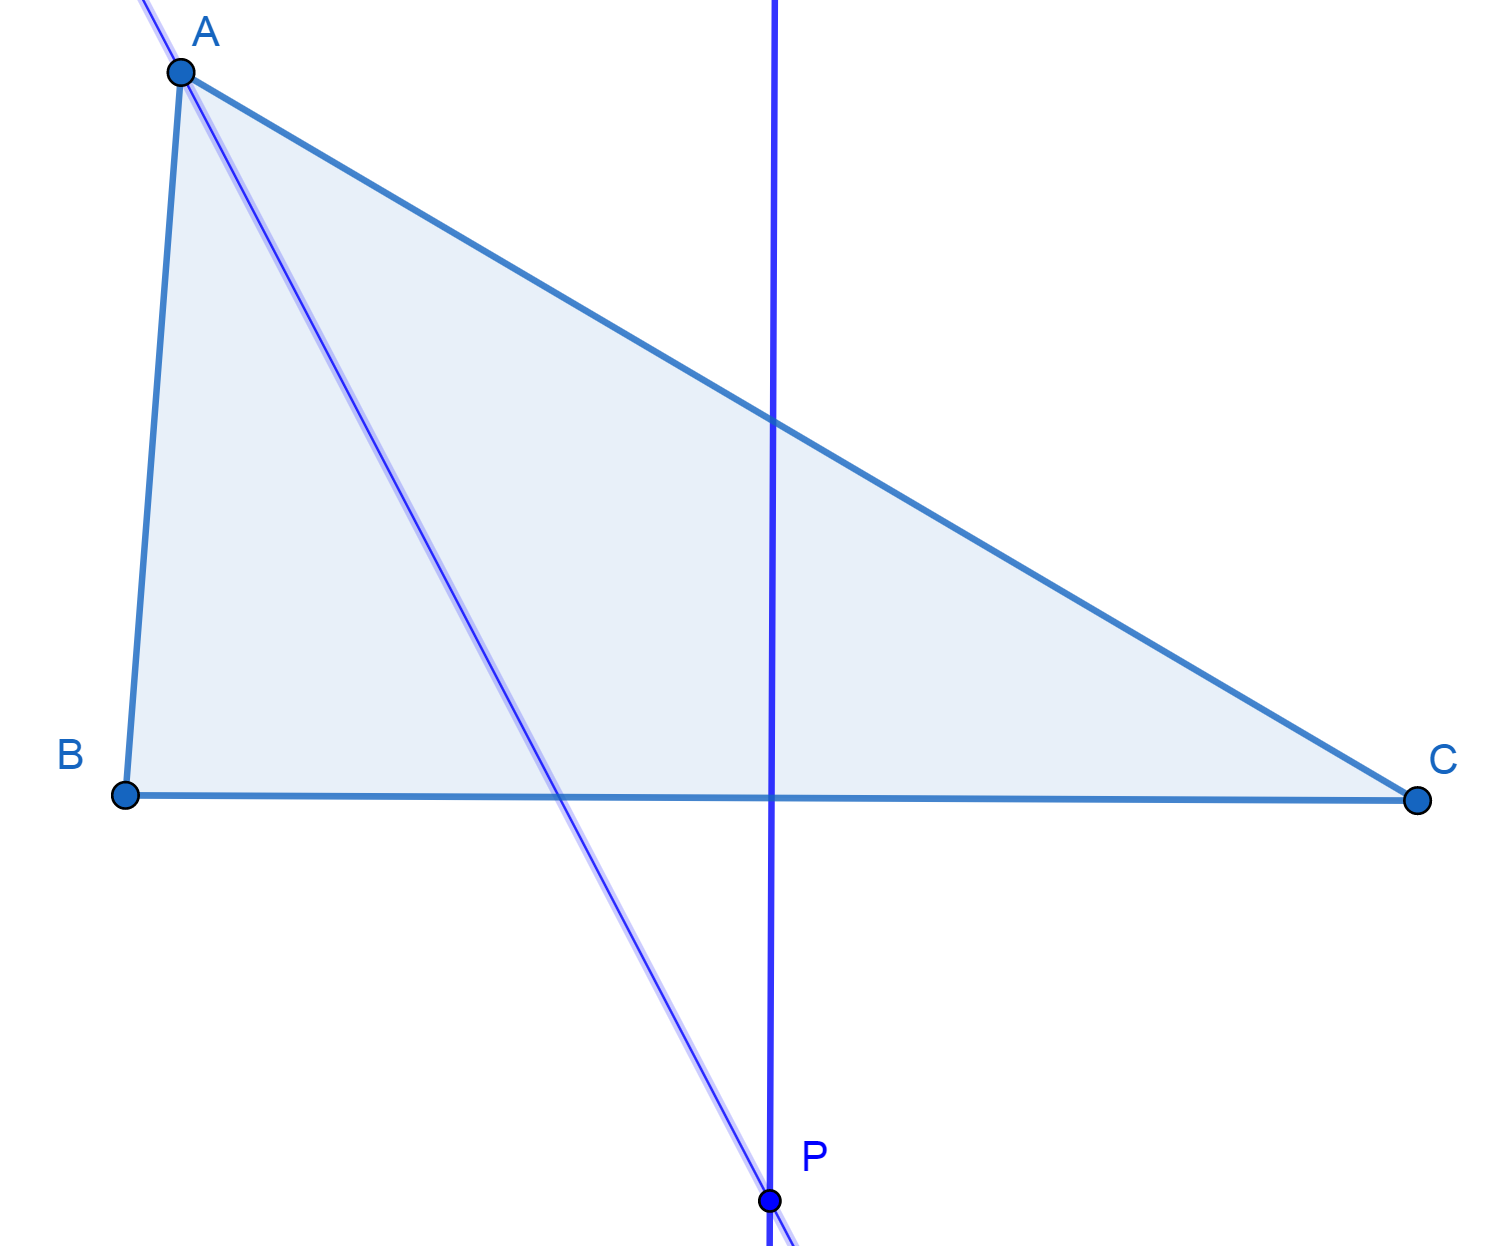
\includegraphics[width=.5\textwidth]{isoceles}
\end{center}

\selectlanguage{english}

%%%%%%%%%%%%%%%%%%%%%%%%%%%%%%%%%%%%%%%%%%%%%%%%%%%%%%%%%%%%%%%
